\section{Graphics Programming in Haskell}

% OpenGL, Gloss etc

\begin{marginfigure}
	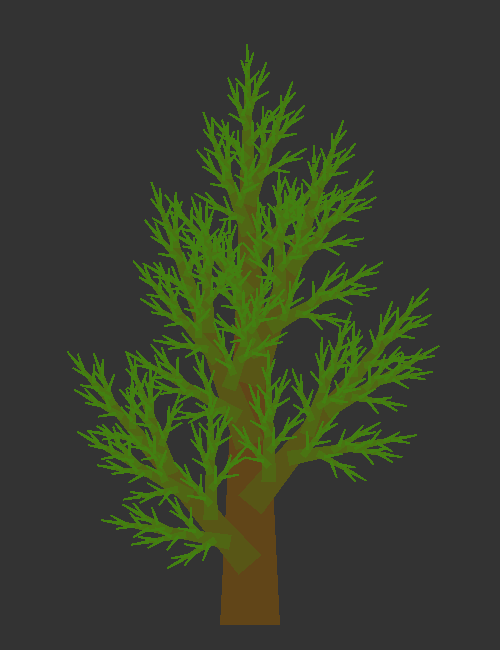
\includegraphics{res/gloss/gloss-tree.png}
	\vspace{1em}
	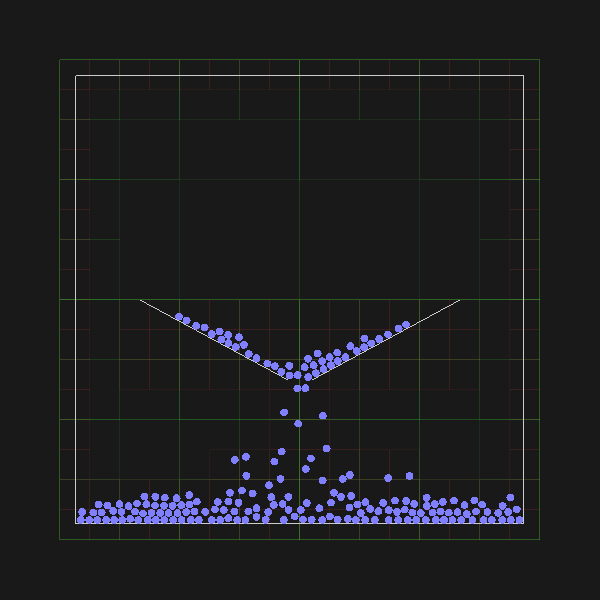
\includegraphics{res/gloss/gloss-styrene.png}
	\caption[Gloss example screens.]{Gloss example screens from \url{gloss.ouroborus.net/}.}
	\label{fig:gloss}
\end{marginfigure}

Any game is clearly going to involve graphics in some capacity or another, but graphics are not something that at first sight seem suited to a functional language. There are, however, various graphical frameworks and bindings available for Haskell.

For the purposes of the Serenity project, the choice basically boiled down to three options. Firstly, there are bindings directly to OpenGl available; which would provide the most flexibility but also likely the most development time. Secondly there are the bindings to the SDL engine, along with all the various tools provided with its framework. Many of the existing games written in Haskell use SDL. Lastly there is the use of the simple but effective layer over GLUT and OpenGL provided by the Gloss library.

This was not an easy decision, and some time went into making it. The direction taken in the Serenity project was to use the Gloss library, mostly because of its simple interface and ease of use, given the limited time and large scope of the rest of the project. The advantages of Gloss can be appreciated by considering the two screens in Figure \ref{fig:gloss}. Both of these examples involve relatively simple code, which is almost entirely pure.

The decision to use Gloss has largely been held up, but there has been some problems due to features it lacks, the most notable being clipping. In the future it would probably be beneficial to replace Gloss with an in house framework providing a layer between the pure graphics code and impure bindings to OpenGL. (This is discussed further in the next section.)

\paragraph{Summary of this section} Given the limited time available for the Serenity project, the prebuilt pure interface onto OpenGL provided by the Gloss library was the best option, and this has been born out by the results. A custom made layer that is more appropriate for the needs of a complex game, and more readily adapted to changing requirements, would be beneficial to develop in the future.
